\documentclass[11pt, a4paper, leqno]{article}
\usepackage{a4wide}
\usepackage[T1]{fontenc}
\usepackage[utf8]{inputenc}
\usepackage{float, afterpage, rotating, graphicx}
\usepackage{epstopdf}
\usepackage{longtable, booktabs, tabularx}
\usepackage{fancyvrb, moreverb, relsize}
\usepackage{eurosym, calc}
% \usepackage{chngcntr}
\usepackage{amsmath, amssymb, amsfonts, amsthm, bm}
\usepackage{caption}
\usepackage{mdwlist}
\usepackage{xfrac}
\usepackage{setspace}
\usepackage[dvipsnames]{xcolor}
\usepackage{abstract}
\usepackage{subcaption}
\usepackage{minibox}
% \usepackage{pdf14} % Enable for Manuscriptcentral -- can't handle pdf 1.5
% \usepackage{endfloat} % Enable to move tables / figures to the end. Useful for some
% submissions.
\usepackage{threeparttable}
\usepackage{multicol}
\usepackage[
    natbib=true,
    bibencoding=inputenc,
    bibstyle=authoryear-ibid,
    citestyle=authoryear-comp,
    maxcitenames=3,
    maxbibnames=10,
    useprefix=false,
    sortcites=true,
    backend=biber,
    doi=false,
    url=false,
    isbn=false,
]{biblatex}

\AtEveryBibitem{
    \clearfield{issn}
    \clearfield{note}
}


\AtBeginDocument{\toggletrue{blx@useprefix}}
\AtBeginBibliography{\togglefalse{blx@useprefix}}
\setlength{\bibitemsep}{1.5ex}
\addbibresource{refs.bib}
\graphicspath{ {./graphs/} }
\usepackage[unicode=true]{hyperref}
\hypersetup{
    colorlinks=true,
    linkcolor=black,
    anchorcolor=black,
    citecolor=NavyBlue,
    filecolor=black,
    menucolor=black,
    runcolor=black,
    urlcolor=NavyBlue
}


\widowpenalty=10000
\clubpenalty=10000

\setlength{\parskip}{1ex}
%\setlength{\parindent}{0ex}
\setstretch{1.5}

\usepackage{acronym}
\acrodef{iid}[i.i.d.]{\textbf{independent and identically distributed}}
\acrodef{did}[DiD]{\textbf{Difference-in-Differences}}
\acrodef{ols}[OLS]{\textbf{Ordinary Least Squares}}
\acrodef{twfe}[TWFE]{\textbf{Two-Way Fixed Effects}}
\acrodef{twfer}[TWFEr]{\textbf{Two-Way Fixed Effects Regression}}
\acrodef{OWFE}[OWFE]{\textbf{One-Way Fixed Effects}}
\acrodef{mcs}[MCS]{\textbf{Monte Carlo Simulation}}
\acrodef{att}[ATT]{\textbf{average treatment effect on the treated}}
\acrodef{pta}[PTA]{\textbf{parallel trends assumption}}
\acrodef{ipw}[IPW]{\textbf{Inverse Probability Weighting}}
\acrodef{drdid}[DRDiD]{\textbf{Doubly-Robust DiD}}
\acrodef{or}[OR]{\textbf{Outcome Regression}}
\acrodef{dgp}[DGP]{\textbf{data generating process}}
\acrodef{mlp}[MLP]{\textbf{multilayer perceptron}}
\acrodef{relu}[ReLU]{\textbf{rectified linear unit}}


\begin{document}


\begin{titlepage}

\begin{center}

\vspace*{0.4cm}

\huge {\bfseries Deep Learning for Semiparametric Difference-in-Difference Estimation}

\vspace{1cm}

\large {Master Thesis Presented to the}\\
\large {Department of Economics at the}\\
\large {Rheinische Friedrich-Wilhelms-Universität Bonn}\\

\end{center}

\vspace{1cm}

\begin{center}


\large {In Partial Fulfillment of the Requirements for the Degree of}\\
\large {Master of Science (M.Sc.)}\\

\end{center}
\vspace{1cm}
\begin{center}

\vspace*{1cm}


\large {Supervisor: Prof. Dr. Christoph Breunig}\\

\end{center}

\vspace{1cm}

\begin{center}

\vfill


\large {Submitted in \today \, by:}\\
\large {Norman Lothar Metzinger}\\
\large {Matriculation Number: 3501090}\\

\end{center}

\vspace{1cm}



\setcounter{page}{0}\clearpage




\end{titlepage}

\endinput

%\input{./abstract.tex}
\thispagestyle{empty}
\begin{abstract}
\noindent This thesis explores the implementation of deep feedforward neural networks into semiparametric Difference-in-Differences estimation (DiD), highlighting its potential under conditional parallel trends assumption.
It reviews current classical and deep learning estimation methods for first-step DiD estimation and conducts a Monte Carlo Simulation to test their validity for second-step inference.
The results demonstrate that deep learning performs nearly as well as the best classical approaches and outperforms those in scenarios with incorrectly specified outcomes.
To further investigate deep learning, multiple deep learning architectures are tested, showing sensitivity towards their hyperparameters.
Finally, DiD deep learning estimators show promise in real-world applications, handling heterogeneous treatment effects effectively.
\end{abstract}
\clearpage
\tableofcontents
\thispagestyle{empty}
\newpage
\setcounter{page}{1}

\section{Introduction}



% Issues and importance of Inference and DIfference in Difference and how Deep Learning could tackle that

\ac{did} is a widely used econometric method to estimate the effect of a policy change on a group of individuals called treatment group.
To achieve this, the method requires to compare treatment group to a control group before and after the policy change.
The important underlying assumption is the \ac{pta}, which states that the treatment and control group would have developed similarly in the absence of the policy change.
This assumption is key to identify the effect on the treatment group, the \ac{att}, to be causal.

However in practice one does not know if the \ac{pta} holds as it is by design untestable.
If individuals are selected into treatment based on characteristics that also influence the outcome, the \ac{pta} is violated.
To overcome this issue researchers condition on these characteristics such that they assume conditional \ac{pta} \citep[see][]{santannaDoublyRobustDifferenceindifferences2020,manfeDifferenceInDifferenceDesignRepeated}

In this thesis I want to adress how researchers can use a more flexible semiparametric approach to achieve robust \ac{did} estimation under conditional \ac{pta}.
For this I consider a variety of machine and deep learning models to interchange the first-step in the \ac{did} estimation.
Especially the use of deep learning marks a novelty and I follow \citet{farrellDeepNeuralNetworks2021} to contribute to the young but growing literature.
% Importance of Deep Learning for Inference and for Economics



% say what the exact finding is in the following parts and keep the structure with First, Second, ... .
%
This thesis wants to contribute in four ways to the literature.
First, I want to discuss the current state of classical and machine learning techniques used for \ac{did} estimation.
For this I revise the classic \ac{did} estimation with \ac{twfe}, then I revise the semiparametric approaches such as \ac{or} \citep[see][]{heckmanMatchingEconometricEvaluation1998}, \ac{ipw} \citep[see][]{abadieSemiparametricDifferenceinDifferencesEstimators2005}, and \ac{drdid} \citep[see][]{santannaDoublyRobustDifferenceindifferences2020}.

Second, I introduce a new approach using deep learning for first step \ac{did} estimation.
As the literature is rather new I want to revise how deep neural networks work and why they can be valid for inference following the results of \citet{farrellDeepNeuralNetworks2021}.
Third, I want to provide a comprehensive \textit{Monte Carlo Simulation} to compare the performance of these techniques. %explain more
Lastly, I want to apply these techniques to a real-world dataset to show the potential of these techniques. %explain more


% Organization of the paper
 % (fold)
\section{Methodology}

\subsection{Notation and Setup}



\subsection{Classic 2x2 Difference in Difference}
%derive the explanation of 2x2 difference in difference from classic to TWFE and talk about heterogeneous effects




\subsection{Outcome Regression}



\subsection{Inverse Probability Weighting}


\subsection{Double Robust Difference in Difference}

\section{Deep Learning}

\subsection{Revision of Deep Learning}
Deep learning is a rapidly developing field within machine learning that has recently received significant attention in economics.
The idea is to transform complex data into a series of simpler representations, each of which is expressed in terms of the previous one \citep{Goodfellow-et-al-2016}.
A common example is the \textit{feedforward neural network} architecture, which consists of a series of layers of neurons, each of which is connected to the next layer.
The first layer is the input layer, the last layer is the output layer, and the layers in between are called hidden layers.
The input layer corresponds to the covariates $X$, the output layer corresponds to the outcome $Y$.
Figure \ref{fig:1} illustrates the layer and node structure of a \ac{mlp}, which is a special class of feedforward networks and is commonly used in empirical applications \citep{farrellDeepNeuralNetworks2021}.
In this thesis, I use the wordings of \ac{mlp}, feedforward neural network, and deep learning interchangeably as these are the approaches used here.

The actual computation within the neural networks is done by the \textit{activation function} $ \sigma : \mathbb{R} \to \mathbb{R} $, which is applied to the output of each hidden neuron.
The most common activation function is the \ac{relu} function, defined as $ \sigma(x) = \max(0, x) $, which is used in this thesis.
The advantage of the linear \ac{relu} is its computational efficiency and its ability to circumvent the vanishing gradient problem, which is a common problem in deep learning \citep{10.1214/19-AOS1875}.\footnote[1]{The vanishing gradient issue arises especially by activation functions like \textit{sigmoid} and \textit{tanh}.
When the neural network model is trained, all the weights of the model are updated through a process called \textit{backpropagation}.
Backpropagation is the algorithm used to compute the gradient of the loss function with respect to each parameter, which is then used to update the parameters such that they minimize the loss.
The issue that can arise is that updating of parameters is hindered or training is completely stopped \citep{abuqaddom2021oriented}.}
The \ac{relu} takes any linear combination given by $\tilde{x}' w + b$ and transforms it to $ \sigma(\tilde{x}' w + b)$, where $w$ is the weight vector, $b$ is the constant term\footnote[2]{The actual term in computer science is \textit{bias} but to avoid confusion with the econometric term I follow \citet{farrellDeepNeuralNetworks2021} and use the term \textit{constant}.}
, and $\tilde{x}$ is the input vector.
Thus, the \ac{relu} function sets all negative values from the linear combination $\tilde{x}' w + b$ to zero, while keeping all positive values unchanged.
An example of a \ac{relu} function is shown in the Appendix Figure \ref{fig:relu}.
\begin{figure}%                 use [hb] only if necceccary!
\centering
\caption{Illustration of a feedforward neural network \citep{farrellDeepNeuralNetworks2021}}
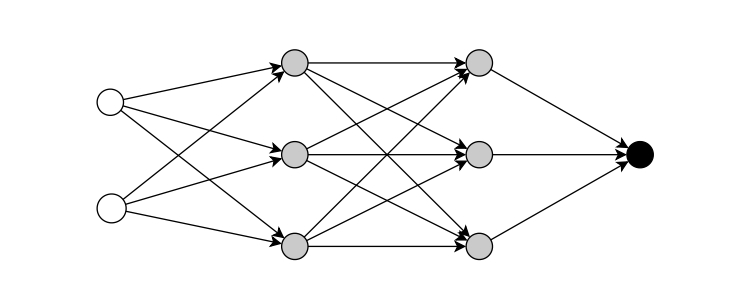
\includegraphics[width=\textwidth]{Neural_net}
\caption*{Note: This figure illustrates the basic structure of a \ac{mlp} $\mathcal{F}_{\text{MLP}}$, showing the input layer with $d=2$ neurons in white. The two ($H=2$) hidden layers in grey with $U=6$ neurons, and one output layer in black ($L=1$). The total amount of weights is $W=25$.}
\label{fig:1}
\end{figure}


The main problem the neural network aims to solve is estimating the unknown function $f^*(x)$.
More precisely, $f^*$ is a function that maps the input $\tilde{x}$ to the output $\tilde{y}$.
As $f^*$ is unknown, the neural network tries to estimate it by minimizing the expected loss function $\mathbb{E}[\ell(f, Z)]$, which can be written as:
\begin{equation}
f^* = \arg \min_f \mathbb{E}[\ell(f, Z)],
\end{equation}
where $\ell(f, Z)$ is the loss function, and the function $f$ predicts the outcome $\hat{Y} = f(X)$ and $Z = (Y, X')' \in \mathbb{R}^{d+1}$ is the set of random variables.
The loss function can take various forms, such as least squares or logistic regression, with the latter used for propensity score estimation in this thesis.
The logistic loss function is therefore defined as follows:
\begin{equation}
f^*(x) := \log \left( \frac{\mathbb{E}[Y|X = x]}{1 - \mathbb{E}[Y|X = x]} \right) \quad \text{and} \quad \ell(f, z) = -yf(x) + \log(1 + e^{f(x)}).
\label{eq:8}
\end{equation}
The logistic regression in eq. \ref*{eq:8} is a method used for binary classification and estimates the probability that the covariates $X$ take on values $0$ or $1$.
The loss function measures the difference between the estimated probabilities and the actual class values.
Unlike simple logistic regression applications, deep learning minimizes the loss function $\ell(f, z)$ by updating iteratively the weights and constants.
For this $Z$ is passed multiple times through the neural network until the loss is minimized.
The amount of iterations is called \textit{epochs}.
Each epoch refers to one complete pass of the training dataset through the neural network.
In practice, multiple epochs are required for the network to minimize the loss function.

Combining all the elements described above, the full neural network can be formalized through recursion:
\begin{equation}
\hat{f}_{\text{MLP}}(x) = W_L \sigma \left( \cdots \sigma \left( W_3 \sigma \left( W_2 \sigma \left( W_1 \sigma \left( W_0 x + b_0 \right) + b_1 \right) + b_2 \right) + b_3 \right) + \cdots \right) + b_L,
\label{eq:9}
\end{equation}
where $\hat{f}$ can be interpreted as a series of nested functions, where each function is a linear combination of the previous function.
Note that $W_l$ is the weight matrix for layer $l$.
Equation \ref{eq:9} shows how the \ac{relu} activation function $sigma$ is applied to each hidden layer, starting with the covariates $x$.
The transformed output of each hidden layer becomes the input for the next layer, and this process continues iteratively until the loss function is minimized.
During this iterative process, the weights $W$ and biases $b$ are adjusted using the gradients computed from the loss function, typically through gradient descent.
This ensures that the network parameters are optimized to improve prediction accuracy.

Equation \ref{eq:10} shows an example of a neural network with $L$ hidden layers and the final output layer:
\begin{align}
h_1 &= \sigma(W_1 X + b_1), \nonumber \\
h_2 &= \sigma(W_2 h_1 + b_2), \nonumber  \\
&\vdots \nonumber \\
h_L &= \sigma(W_L h_{L-1} + b_L),
\label{eq:10}
\end{align}
Finally, the output of the network is:
\begin{equation}
\hat{Y} = W_L h_{L-1} + b_L, \nonumber
\end{equation}



Some final remarks on neural networks in general.
First, if deep learning practitioners mention tuning parameters then they refer to adjusting the width and depth of the network, e.g. the amount of hidden layers \citep{farrellDeepNeuralNetworks2021}.
These parameters are also the ones on which the neural network is repeatedly trained.
Secondly, unlike inference, there is no understanding within the deep learning literature on how to select the optimal architecture or tuning parameters \citep[see][]{10.1214/19-AOS1875,telgarsky2016benefits}.
Consequently, the chosen neural network architecture may not be the optimal one, and selecting the right architecture is often arbitrary.
\subsection{Deep Learning for Inference}
%first cite farrel paper where they describe the two use cases of semiparametric ML stuff
The recent applications of deep learning for inferences mostly focus on prediction problems, such as outcome or propensity score prediction.
The idea is to embed the neural network within a semiparametric framework, where the neural network is used to estimate the unknown function $f^*$.
In this framework, the neural network is used as a first-step estimator, where the fitted values estimated by the neural network are used as the input for the second-step inference. %is this correct?
Other techniques such as tree-based methods, logistic regression, or hybrid models are also used as first-step estimators.
The advantage of these machine learning approaches is their robustness towards heterogeneous treatment effects, conditional controls, or many covariates \citep{belloni2017program}.
\citet{belloni2017program} shows that neural networks perform as well as other machine learning approaches in terms of recovering the true treatment effect as a first-step estimator.
\citet{chernozhukovDoubleDebiasedMachine2018} approves those results in a low-dimensional setting but reports issues with the neural network if $n$ is small.
Common across literature are the benefits of deep learning regarding handling heterogeneous treatment effects \citep[see][]{DeepLearningIndividual2021,belloni2017program,chernozhukovDoubleDebiasedMachine2018}

Another advantage of Deep learning is its effectiveness in high covariate settings \citep{chernozhukov2022automatic}.\footnote[3]{\citet{belloni2017program} demonstrate this for \textit{moderately high} and \textit{very high} amount of covariates compared to the sample size.}
This advantage arises from deep learning's capability to perform variable selection.
Especially employing some form of regularization, deep learning can reduce the variance induced by high covariates, albeit at the cost of increased bias \citep{chernozhukovDoubleDebiasedMachine2018}.
Many machine learning techniques (e.g., lasso or certain tree-based methods) have similar properties.
As such this thesis does not try to promote deep learning as an optimal technique but aims to investigate its utility as a valid first-step estimator in a semiparametric \ac{did} framework.

To evaluate deep learning performance there are multiple important criteria to consider.
First, deep learning should have good approximation power \citep{belloni2017program}, meaning it can closely approximate the true underlying function of the data.
Second, deep learning should avoid overfitting the data \citep{belloni2017program}, leading to poor generalization of new data.
%explain what that means and how one can see that
Third, \citet{belloni2017program} emphasize that doubly robust estimation methods ensure valid inference for many machine learning frameworks, including neural networks.\footnote[4]{\citet{belloni2017program} also point out that some form of orthogonal moment condition can also lead to valid inference in this setting. See \citet{DeepLearningIndividual2021} for a discussion that with even weaker conditions than doubly robust or orthogonality valid semiparametric inference is achievable, although these are not of focus here.}

\section{Monte Carlo Simulations}


\subsection{Data Generating Process}

In this section, I present the data \ac{dgp} for the Monte Carlo simulations.
The \ac{dgp} is based on the simulation study by \citet{kang2007demystifying} and \citet{santannaDoublyRobustDifferenceindifferences2020}.
The advantage of this setup is to ensure comparability with previous studies and allowing to validate novel approaches as the use of deep learning for \ac{did} estimation.
For all simulations, the \ac{dgp} has a total sample size of $n=1000$.
There are two time periods $t=0,1$ and two groups $i=0,1$ investigated, such that it allows to apply the classical $2\times2$-\ac{did} estimator.
As individuals are tracked over time, the data is panel data.
\citet{kang2007demystifying} created the \ac{dgp} the way such there are covariate specific trends and homogenous treatment effects.
In the first simulation in Table \ref{tab:table1} I stick to this specification, in the second simulation in Table \ref{tab:table2} I extend the \ac{dgp} to allow for heterogeneous treatment effects.

Consider the arbitrary input vector $M = (M_1, M_2, M_3, M_4)'$ and let the true \ac{or} and \ac{ipw} model be defined as follows:
\begin{align}
    f_{\text{or}}(M) &= 210 + 27.4 \cdot M_1 + 13.7 \cdot (M_2 + M_3 + M_4), \\
    f_{\text{ipw}}(M) &= 0.75 \cdot (-M_1 + 0.5 \cdot M_2 - 0.25 \cdot M_3 - 0.1 \cdot M_4).
\end{align}
Note that in this data is a selection bias constructed \citep{kang2007demystifying} such that naive estimators are likely to be biased.
As $M$ is arbitrary, \citet{kang2007demystifying} introduce two variations of covariates $Z$ and $X$ that are used in the simulations.
$Z$ is a set of observable variables, while $X$ is a set of unobservable variables.
In this simulation study, $f_{\text{or}}(M)$ and $f_{\text{ipw}}(M)$ is constructed only by $Z$ or only by $X$ or a combination of both.
Thus there are four different \ac{dgp} setups that are labeled as DGP1, DGP2, DGP3, and DGP4.
These four setups differ because $Z$ is a non-linear transformation of $X$.

Consider $\mathbf{X} = (X_1, X_2, X_3, X_4)'$ be distributed as $N(0, I_4)$. $I_4$ is the $4 \times 4$ identity matrix.
For $j = 1, 2, 3, 4$, \citet{kang2007demystifying} define the following variations of $Z_j = \frac{\tilde{Z}_j - \mathbb{E}[\tilde{Z}_j]}{\sqrt{\text{Var}(\tilde{Z}_j)}}$ where
\begin{align} \nonumber
\tilde{Z}_1 &= \exp(0.5X_1), \\ \nonumber
\tilde{Z}_2 &= 10 + \frac{X_2}{1 + \exp(X_1)}, \\
\tilde{Z}_3 &= (0.6 + \frac{X_1 X_3}{25})^3, \quad \text{and} \\ \nonumber
\tilde{Z}_4 &= (20 + X_2 + X_4)^2.  \nonumber
\label{eq:13}
\end{align}
Each variation of $Z$ differs by their functional form as they are quadratic, exponential, and cubic,
They also include variations of interactions of $X$.
This complexity in the functional form of $Z$ is added to invoke potential biases, when estimating the \ac{att}.
For example, when the true \ac{dgp} is based on $X$ but the model estimates based on $Z$ then the estimates are likely to be biased.
As we can construct either the \ac{or} or \ac{ipw} model based on $Z$ or $X$ or a combination of both, we have four different setups.
In the following is the setup for each \ac{dgp} presented and it is also stated which model is then correctly specified and which is not.
\begin{multicols}{2}

\textbf{DGP1} \\
(IPW and OR models correct)
\begin{align*}
    Y_0(0) &= f_{\text{or}}(Z) + \nu(Z, D) + \epsilon_0, \\
    Y_1(d) &= 2 \cdot f_{\text{or}}(Z) + \nu(Z, D) + \epsilon_1(d) \\
    p(Z) &= \frac{\exp \left( f_{\text{ipw}}(Z) \right)}{1 + \exp \left( f_{\text{ipw}}(Z) \right)}, \\
    D &= 1\{ p(Z) \geq U \};
\end{align*}

\textbf{DGP2} \\
(IPW model incorrect, OR correct)
\begin{align*}
    Y_0(0) &= f_{\text{or}}(Z) + \nu(Z, D) + \epsilon_0, \\
    Y_1(d) &= 2 \cdot f_{\text{or}}(Z) + \nu(Z, D) + \epsilon_1(d) \\
    p(X) &= \frac{\exp \left( f_{\text{ipw}}(X) \right)}{1 + \exp \left( f_{\text{ipw}}(X) \right)}, \\
    D &= 1\{ p(X) \geq U \};
\end{align*}

\columnbreak

\textbf{DGP3}\\
(IPW model correct, OR incorrect)
\begin{align*}
    Y_0(0) &= f_{\text{or}}(X) + \nu(X, D) + \epsilon_0, \\
    Y_1(d) &= 2 \cdot f_{\text{or}}(X) + \nu(X, D) + \epsilon_1(d) \\
    p(Z) &= \frac{\exp \left( f_{\text{ipw}}(Z) \right)}{1 + \exp \left( f_{\text{ipw}}(Z) \right)}, \\
    D &= 1\{ p(X) \geq U \};
\end{align*}

\textbf{DGP4 } \\
(IPW and OR models incorrect)
\begin{align*}
    Y_0(0) &= f_{\text{or}}(X) + \nu(X, D) + \epsilon_0, \\
    Y_1(d) &= 2 \cdot f_{\text{or}}(X) + \nu(X, D) + \epsilon_1(d) \\
    p(X) &= \frac{\exp \left( f_{\text{ipw}}(X) \right)}{1 + \exp \left( f_{\text{ipw}}(X) \right)}, \\
    D &= 1\{ p(X) \geq U \};
\end{align*}

\end{multicols}

\subsection{Results Homogenous Treatment Effects}

\begin{table}[htbp]
\centering
\resizebox{\linewidth}{!}{
\begin{threeparttable}
\caption{Monte Carlo Simulation with Homogenous Treatment Effects}
\label{tab:table1}
\begin{tabular}{lllllll}
\toprule
\hline
\addlinespace
Estimator         & Reference                         & Av. Bias   & Med. Bias   & RMSE & Variance & Cover \\ \midrule
\addlinespace
\large \textbf{DGP1}            &                                   &            &             &      &           \\
\addlinespace
$\hat{\tau}^{fe}$ & Regression, Eq. \eqref{eq:twfe}               & -20.963       & -20.816        & 21.277 & 13.247& 0.000      \\
$\hat{\tau}^{corr}$ & Regression, Eq. (2)             & -0.002       & -0.001        & 0.196 & 0.038  &  0.840   \\
$\hat{\tau}^{ipw}$ & Abadie (2005)                    & -0.376       & -0.469        & 9.396 & 45.704 &  0.840      \\
$\hat{\tau}^{ipw,dl}$ & Abadie (2005) + DL            & -3.819       & -3.697        & 3.841 & 36.065 &  1.000    \\
$\hat{\tau}^{dr}$ & Sant'Anna and Zhao (2020)         & 0.003      & 0.008       & 0.218 & 0.022  &  0.834   \\
$\hat{\tau}^{dr,dl}$ & Sant'Anna and Zhao (2020) + DL & -0.121       & -0.120        & 0.121 & 0.020  & 1.000    \\\midrule


\addlinespace
\large \textbf{DGP2}            &                                   &            &             &      &           \\
\addlinespace
$\hat{\tau}^{fe}$ & Regression, Eq. \eqref{eq:twfe}               & -19.261      & -19.040      & 19.606 & 13.403 & 0.000      \\
$\hat{\tau}^{corr}$ & Regression, Eq. (2)             & -0.004       & -0.001        & 0.195 & 0.038  & 0.832     \\
$\hat{\tau}^{ipw}$ & Abadie (2005)                    & -0.498       & -0.472        & 9.660 & 47.106  & 0.839    \\
$\hat{\tau}^{ipw,dl}$ & Abadie (2005) + DL            & -21.983       & -22.114        & 22.335 & 43.872 & 0.000    \\
$\hat{\tau}^{dr}$ & Sant'Anna and Zhao (2020)         & 0.005       & 0.002        & 0.207 & 0.021  & 0.802    \\
$\hat{\tau}^{dr,dl}$ & Sant'Anna and Zhao (2020) + DL  & -0.148       & -0.150        & 0.148 & 0.020  &  1.000    \\  \midrule


\addlinespace
\large \textbf{DGP3}            &                                   &            &             &      &           \\
\addlinespace
$\hat{\tau}^{fe}$ & Regression, Eq. \eqref{eq:twfe}               & 13.122       & 12.899       & 14.028 & 24.575 & 0.109    \\
$\hat{\tau}^{corr}$ & Regression, Eq. (2)             & 0.142       & -0.114       & 4.869 & 23.685 &0.782   \\
$\hat{\tau}^{ipw}$ & Abadie (2005)                    & 0.109     & 0.219      & 9.630 & 43.498  & 0.817   \\
$\hat{\tau}^{ipw,dl}$ & Abadie (2005) + DL            & -0.810       & -0.794        & 0.824 & 40.227  &   1.000  \\
$\hat{\tau}^{dr}$ & Sant'Anna and Zhao (2020)         & -0.104       & 0.052        & 4.599 & 11.165  &0.840    \\
$\hat{\tau}^{dr,dl}$ & Sant'Anna and Zhao (2020) + DL & 0.228       & 0.219        & 0.293 & 11.240   &1.000   \\  \midrule


\addlinespace
\large \textbf{DGP4}            &                                   &            &             &      &           \\
\addlinespace
$\hat{\tau}^{fe}$ & Regression, Eq. \eqref{eq:twfe}              & -16.434       & -16.283        & 17.226 & 26.633  & 0.033   \\
$\hat{\tau}^{corr}$ & Regression, Eq. (2)             & -3.063       & -3.165       & 6.162 & 28.588  &0.654   \\
$\hat{\tau}^{ipw}$ & Abadie (2005)                    & -3.881       & -4.063        & 10.576 & 47.230    & 0.798  \\
$\hat{\tau}^{ipw,dl}$ & Abadie (2005) + DL            & -4.992       & -4.962        & 5.005 & 43.947 & 1.000     \\
$\hat{\tau}^{dr}$ & Sant'Anna and Zhao (2020)         &-3.177      &-3.162       & 5.899 & 12.259  &0.752    \\
$\hat{\tau}^{dr,dl}$ & Sant'Anna and Zhao (2020) + DL & 1.630       & 1.593        & 1.652 & 15.876  &1.000    \\


\bottomrule
\end{tabular}
\vspace{1em}
\begin{tablenotes}
\item Notes: Simulations based on panel data with sample size $n = 1000$ and 1000 Monte Carlo repetitions. The average bias "Av. Bias", median bias "Med. Bias", root mean squared error "RMSE", and average variance "Variance" of the estimators are reported. The "Cover" describes the coverage probability of how often the estimated treatment coefficient falls within the confidence intervall of the true treatment effect. The methods that predict propensity scores with deep learning are marked by "DL". The true treatment effect is $\tau = 0$ in all cases and homogenous.
\end{tablenotes}
\end{threeparttable}}
\end{table}


In this section I present the results of the Monte Carlo simulations for the homogenous treatment effects.
Note that the results in Table \ref{tab:table1}  and Table \ref{tab:table3} report the average bias, median bias, root mean squared error, and variance of the estimators.





\subsection{Results Heterogeneous Treatment Effects}
To explore the flexibility of neural networks, I consider the following data generating processes. Note that this is an adjusted version of the DGP4, where the PS and OR are incorrect and heterogenous treatment effects are added. In \\
\textbf{DGP4 with Heterogeneous Treatment Effects}
\begin{align*}
    Y_0(0) &= f_{\text{or}}(X) + \nu(X) + \epsilon_0, \\
    Y_1(d) &= 2 \cdot f_{\text{or}}(X) + \nu(X) + \theta(X) \cdot d + \epsilon_1(d), \\
    p(X) &= \frac{\exp \left( f_{\text{ps}}(X) \right)}{1 + \exp \left( f_{\text{ps}}(X) \right)}, \\
    D &= 1\{ p(X) \geq U \},
\end{align*}
where: $\theta(X) = 10 \cdot (Z_1 + Z_2 - Z_3 + Z_4)$.
\begin{table}[]
\centering
\begin{threeparttable}
\caption{Monte Carlo Simulation with Heterogenous Treatment Effects in DGP4}
\label{tab:table2}
\begin{tabular}{lllllll}
\toprule
\hline
\addlinespace
Estimator         & Reference                         & Av. Bias   & Med. Bias   & RMSE & Variance & Cover \\ \midrule
\addlinespace
$\hat{\tau}^{fe}$ & Regression, Eq. \eqref{eq:twfe}               & -20.418      & -20.245        & 21.242 & 34.360  &0.015   \\
$\hat{\tau}^{corr}$ & Regression, Eq. \eqref{eq:twfecorr}           & -9.429      & -9.355       & 10.602 & 23.483  &0.225  \\
$\hat{\tau}^{ipw}$ & Abadie (2005)                    & -7.866       & -7.899       & 13.231 & 55.196   &0.712  \\
$\hat{\tau}^{ipw,dl}$ & Abadie (2005) + DL            & -8.424       & -8.408        & 8.432 & 51.123   &1.0   \\
$\hat{\tau}^{dr}$ & Sant'Anna and Zhao (2020)         & -7.238      & -7.128        & 10.115 & 24.060   & 0.619   \\
$\hat{\tau}^{dr,dl}$ & Sant'Anna and Zhao (2020) + DL & -1.596       & -1.607        & 1.633 & 16.570   & 1.0  \\

\bottomrule
\end{tabular}
\begin{tablenotes}
    \item Notes: Simulations based on panel data with sample size $n = 1000$ and 1000 Monte Carlo repetitions. The average bias "Av. Bias", median bias "Med. Bias", root mean squared error "RMSE", and average variance "Variance" of the estimators are reported. The methods that predict propensity scores with deep learning are marked by "DL". The true treatment effect is $\tau = 0$ and heterogenous in all cases.
\end{tablenotes}
\end{threeparttable}
\end{table}



\subsection{Deep Learning Model Results}
[refer to section 3.1 how the loss functions are computed]



% Please add the following required packages to your document preamble:
% \usepackage{booktabs}
% Please add the following required packages to your document preamble:
% \usepackage{booktabs}
\begin{table}[ht]
\centering
\begin{threeparttable}
\caption{Performance of the Neural Network across DGPs}
\label{tab:table3}
\begin{tabular}{ccccc} %\begin{tabular}{@{}lllll@{}}
\toprule
\hline
\addlinespace
Minimum Loss  & DGP1 & DGP2 & DGP3 & DGP4 \\ \midrule
Training   & 0.634 & 0.631 & 0.634 & 0.632 \\
Validation  & 0.617 & 0.626 & 0.617 & 0.625 \\ \bottomrule
\end{tabular}
\begin{tablenotes}
    \item Notes: The neural networks width is set to 32. The depth is set to 3 and the learning rate is set to 0.01. The number of epochs to 50. This specifications are set across all DGPs for the same neural network.
\end{tablenotes}
\end{threeparttable}
\end{table}


\section{Application}

An early application of \ac{did} is the paper of \citet{meyer1990workers} who investigate the effect of workers' compensation on their time out of work.
In 1980, the states of Kentucky and Michigan substantially increased the compensations in case of work-induced disability or injury.
As the policy affected high-earning workers, \citet{meyer1990workers} took low-earning workers as a control group.
Their idea was that low- and high-earning workers are comparable except that high-earning workers are treated with the compensation policy.
The distribution of the pre-treatment compensation duration for low- and high-earning workers can be seen in the Appendix Figure \ref{fig:log_duration_distribution}.
In their original study, they report a significant increase in time out of work for Kentucky but not for Michigan.

\citet{meyer1990workers} implemented a classical $2 \times 2$ \ac{did} design, which makes it suitable to the methods discussed in this thesis.
Due to the low sample size of the Michigan data, the analysis is solely focused on Kentucky.
Therefore, the \ac{did} identification strategy can be formulated as follows:
\begin{equation}
\text{Duration}_{it} = \alpha + \beta_1 \text{Post}_t + \beta_2 \text{HighEarnings}_i + \beta_3 (\text{Post}_t \times \text{HighEarnings}_i) + \gamma X_{it} + \epsilon_{it},
\label{eq:duration}
\end{equation}
where the interaction $(\text{Post}_t \times \text{HighEarnings}_i)$ is the \ac{did} estimator.
$X_{it}$ is a vector of control variables such as injury type, age, or gender.
As \citet{meyer1990workers} use many of these pre-treatment covariates like age or gender it implicates that they assume conditional \ac{pta}.
By design, it is not possible to test for \ac{pta} but the conditional \ac{pta} seems to be a more robust assumption in an observational study \citep{santannaDoublyRobustDifferenceindifferences2020}.
A second remark is towards heterogeneity in the treatment group, which is given in almost all contexts \citep{DeepLearningIndividual2021}.
The Appendix Table \ref{tab:duration} shows the difference in duration of out-of-work time across injury types before and after the treatment.
The magnitude of the differences is quite large, hinting towards heterogeneity in the treatment group.
Based on that, I conducted a regression exclusion test following \citet{hansen2022econometrics} where the results can be seen in Table \ref{tab:exclusion_test} in the Appendix.
The regression exclusion test is significant, which implies that homogeneous treatment effects cannot be assumed.

These results are reason to apply the \ac{drdid} + DL\footnote[5]{Here I use the prebuilt software implementation of \citet*{doubleml2024R} to be able to report summary statistics for the \ac{drdid} + DL estimation.} estimator to the data of \citet{meyer1990workers}.
To compare different designs, I also estimate a saturated dummy design without controls and the regression equation \ref{eq:duration} with controls and interactions.
The estimates are reported in Table \ref{tab:reg_results}.
Note that the results of the regression equation \ref{eq:duration} are slightly different from the results of \citet{meyer1990workers}.
This should be due to different handling of the data-cleaning process than to the different estimation methods.

\begin{table}[ht]
\centering
\begin{threeparttable}
\caption{Regression Results}
\label{tab:reg_results}
\begin{tabular}{lcccccc}
\toprule
\hline
\addlinespace
Model & Coef. & Std.Err. & t & P>|t| & [0.025 & 0.975] \\
\midrule
Saturated design & 0.191 & 0.069 & 2.782 & 0.005 & 0.056 & 0.325 \\
Regression Eq. (14)  & 0.172 & 0.064 & 2.694 & 0.007 & 0.047 & 0.297 \\
\ac{drdid} + DL & 0.250 & 0.075 & 3.34 & 0.000 & 0.103 & 0.396\\
Authors' model & 0.162 & 0.059 &  2.745 & 0.006 & 0.046 & 0.278 \\
\bottomrule
\end{tabular}
\begin{tablenotes}
    \item Notes: In this table are reported the results of a saturated dummy design without controls, the regression equation (14) with controls and interactions, the \ac{drdid} with deep learning and controls and the results from \citet{meyer1990workers} of Table 6 Column (ii). Reported are the coefficients as the \ac{att}, the standard errors, the t-values, P>|t| is the p-value, and the lower- and upper bound of the 95 percent confidence interval. The dependent variable is the log of the duration of work leave. The dataset is taken from the online resources of \citet{wooldridge2019introductory}. The sample size is $n = 5347$.
\end{tablenotes}
\end{threeparttable}
\end{table}


In Table \ref{tab:reg_results}, one can see that the results for all parametric models are quite similar.
Note that the saturated design is similar to the regression equation \ref{eq:duration} implying that the controls might not have a large impact on the results.
Assuming a homogenous treatment effect this result would normally imply that the parametric model is robust and sufficient for estimation.
Due to the potential heterogeneity in the treatment group, the \ac{drdid} + DL estimator is arguably the most robust model.
One can see that the \ac{drdid} + DL estimator is still able to retrieve significant results as the other models, even though the standard errors are slightly larger.
The magnitude of the \ac{att} is also larger than in the other models, implying an even bigger effect of compensation policy in Kentucky than previously assumed.

Even though the \ac{drdid} + DL is more robust to unspecified models and heterogeneity in the treatment group, there is the potential issue of overfitting.
Note that the neural network used in Table \ref{tab:reg_results} has the same architecture as in the simulation study.
Contrary to the simulation study, the neural network reports in this application a higher validation loss ($0.467$) than training loss ($0.445$).
Even though the size of the difference is small, it is a hint towards overfitting.
Arguably the issue of heterogenous treatment effects is more severe than the issue of overfitting.

Finally, the results of the \ac{drdid} + DL estimator are quite promising in observational studies.
In settings with large $n$, conditional \ac{pta}, and potential heterogeneity in the treatment group, the \ac{drdid} + DL estimator seems to be a robust and efficient alternative.

\section{Further Research}


This thesis cannot do justice to all aspects of semiparametric estimation with deep learning, such that there are multiple ways to extend the results in further research.
One possible extension is to apply the aforementioned methods to repeated cross-sectional data.
Although panel data is the preferred data structure for causal inference due to its generally lower variance, cross-sectional data is often the only available option \citep{wooldridge2010econometric}.
Nonetheless, \citet{santannaDoublyRobustDifferenceindifferences2020} and \citet{manfeDifferenceInDifferenceDesignRepeated} demonstrate the usefulness of implementing \ac{did} on repeated cross-sectional data.
Applying deep learning to this data structure could be a promising approach to estimating causal effects.

%santana and callaway how to implement it for multiple time periods
Another extension is to move away from the classical 2x2 \ac{did} setting and apply the deep learning approach to multiple periods or groups.
A natural extension would be the use of the work of \citet{callawayDifferenceinDifferencesMultipleTime2021}, which extend the results of \citet{santannaDoublyRobustDifferenceindifferences2020} that form the basis of this thesis.
The main contributions of  \citet{callawayDifferenceinDifferencesMultipleTime2021} are the application of the \ac{or}, \ac{ipw}, and \ac{drdid} methods to multiple periods and groups.
Accounting for conditional \ac{pta} and heterogenous treatment effect in this setting would make the application of deep learning particularly interesting.

The work of \citet{dechaisemartinDifferenceinDifferencesEstimatorsIntertemporal2024} would be another interesting extension to apply deep learning.
Similar to \citet{callawayDifferenceinDifferencesMultipleTime2021}, they extend the \ac{did} estimator to multiple periods and groups but focus on non-binary, non-absorbing treatments with lags.

%discuss the shortcoming of my results
%overfitting on L2 regularization
%which archtiecture to choose
%more understanding of the inherent structure of the data (like in the farrell paper l2 regularization)
A major criticism of the deep learning approach is the arbitrary choice of architecture and hyperparameters.
There is still a lack of understanding of the inherent structure of deep learning and how to choose the right architecture.
It is unclear how the number of hidden layers, the number of neurons, or the choice of activation function impacts the results.
\citet{farrellDeepNeuralNetworks2021} discuss the unclear effect of l2 regularization on deep learning in inference, even though often used in practice.
In Section 4.4, I discuss that the choice of hyperparameters can influence the magnitude of the results.
More research needs to be done to give guidance on how to choose the right architecture and hyperparameters for deep learning in causal inference.

Even though it is unclear how the size of the architecture influences the outcome of the neural network, the more hidden layers and neurons a neural network has, the more computationally costly it is \citep{thompson2020computational}.
For economists, this issue has been a minor concern in the past, but with the advent of deep- and machine learning, it has become more important.
Especially for large and complex data sets, the computational cost of deep learning can be demanding and computation time extensive.
Further research is needed to understand how to make deep learning computationally more efficient as suggested by \citet{farrellDeepNeuralNetworks2021}.

%what is new stuff
%%ausblick auf neue deep learning approaches (direct estimation with deepl by farrel paper 2)
Finally, a relatively new approach using deep learning for inference is the direct estimation of treatment effects.
Instead of incorporating deep learning within a semiparametric framework, it is used directly to recover parameter functions, as suggested by the work of \citet{DeepLearningIndividual2021}.
This approach allows for second-stage inference, such as estimating how treatment impacts evolve over time or across different subgroups.
Incorporating direct estimation of \ac{att} with deep learning, rather than using it solely for first-stage estimation, could provide an interesting extension for estimating causal effects.

\section{Conclusion}

In this thesis, I have pres

\clearpage


\pagenumbering{Roman}
\section*{Appendix}



\begin{figure}[h]
\centering
\caption{Example of \ac{relu} Activation Function}
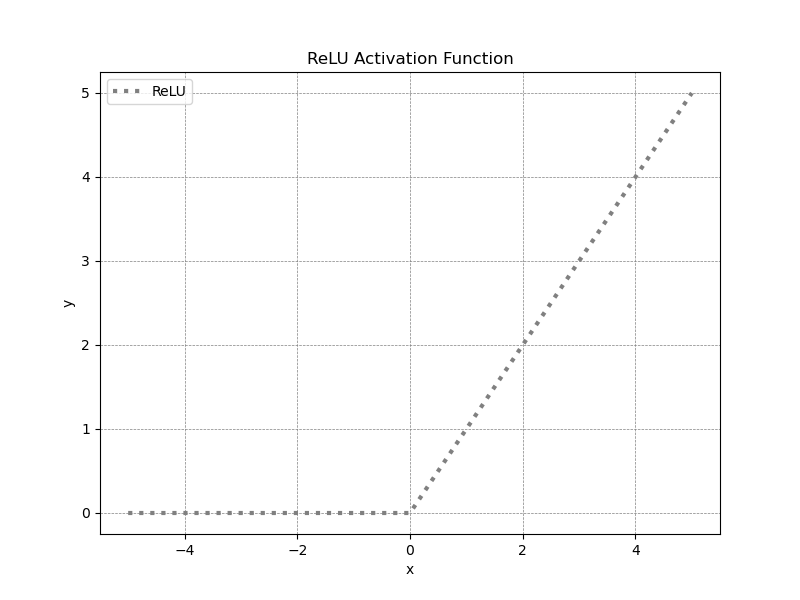
\includegraphics[width=\textwidth]{relu}
\label{fig:relu}
\end{figure}



\begin{figure}[h]
\centering
\caption{Distribution of Log Duration by Earnings Category}
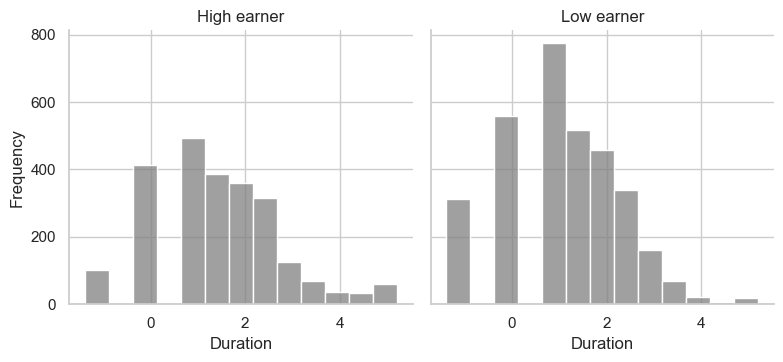
\includegraphics[width=\textwidth]{dist}
\label{fig:log_duration_distribution}
\end{figure}




\begin{table}[ht]
\centering
\caption{Comparison of Duration Across Injury Types Before and After 1980}
\label{tab:duration}
\begin{threeparttable}
\begin{tabular}{ccccccccc}
Injury Type & \textbf{1} & \textbf{2} & \textbf{3} & \textbf{4} & \textbf{5} & \textbf{6} & \textbf{7} & \textbf{8} \\
\hline
\hline
\addlinespace
after\_1980 = 0 & 778.25 & 282.00 & 1993.75 & 1663.25 & 5806.0 & 2649.75 & 194.25 & 413.5 \\
after\_1980 = 1 & 771.50 & 815.25 & 2341.75 & 1997.75 & 5362.5 & 2816.25 & 305.00 & 559.5 \\
Difference & -6.75 & 533.25 & 348.00 & 334.50 & -443.5 & 166.50 & 110.75 & 146.0 \\ \addlinespace
\end{tabular}
\begin{tablenotes}
\small
\item \textbf{Notes:}
\item \textbf{Injury Type}: Categories of injuries.
\item \textbf{after\_1980 = 0}: Duration of work leave before 1980.
\item \textbf{after\_1980 = 1}: Duration of work leave  after 1980.
\item \textbf{Difference}: Difference in duration values between after\_1980 = 1 and after\_1980 = 0.
\end{tablenotes}
\end{threeparttable}
\end{table}


% Please add the following required packages to your document preamble:
% \usepackage{graphicx}
\begin{table}[]
\centering
\caption{Regression Exclusion Test}
\label{tab:exclusion_test}
\resizebox{\columnwidth}{!}{%
\begin{tabular}{llllll}
Residual Degrees & Sum of Squared  & Degrees of  & Sum of Squares& F     & Pr(\textgreater{}(F)) \\
of Freedom                    &   Residuals                       &     Freedom Difference                          &         Difference                    &       &                       \\
\hline
\hline
\addlinespace
\addlinespace
2385.0           & 1.927912e+06             & 7.0                           & 32812.658                 & 5.798 & 0.000  \\ \addlinespace
\end{tabular}%
}
\begin{tablenotes}
    \small
    \item \textbf{Notes}:
    \item The table reports the results of the regression exclusion test. The test compares the full model with the restricted model, excluding the variable of interest.
    \small\item \textbf{Residual Degrees of Freedom}: Number of independent pieces of information remaining after fitting the model.
    \small\item \textbf{Sum of Squared Residuals}: Measure of the discrepancy between the observed data and the model's predictions, quantifying the variation not explained by the model.
    \small\item \textbf{Degrees of Freedom Difference}: Change in the degrees of freedom when moving from the restricted model to the full model.
    \small\item \textbf{Sum of Squares Difference}: Reduction in the sum of squared residuals when additional variables are added, indicating the improvement in model fit.
    \small\item \textbf{F}: F-statistic for the comparison of the two models.
    \small \item \textbf{Pr(>F)}: p-value for the F-test, indicating the significance of the difference between the models.
    \end{tablenotes}
\end{table}

\clearpage

\printbibliography



\clearpage
"I hereby confirm that the work presented has been performed and
interpreted solely by myself except for where I explicitly identified the
contrary. I assure that this work has not been presented in any other
form for the fulfillment of any other degree or qualification. Ideas
taken from other works in letter and in spirit are identified in every
single case."

\today %\begin{flushright} \begin{tabular}{l@{}} Norman Metzinger \end{tabular} \end{flushright}
\\
\\
Norman Metzinger




% \appendix

% The chngctr package is needed for the following lines.
% \counterwithin{table}{section}
% \counterwithin{figure}{section}

\end{document}
